% $Header$

\documentclass{beamer}

% This file is a solution template for:

% - Talk at a conference/colloquium.
% - Talk length is about 20min.
% - Style is ornate.



% Copyright 2004 by Till Tantau <tantau@users.sourceforge.net>.
%
% In principle, this file can be redistributed and/or modified under
% the terms of the GNU Public License, version 2.
%
% However, this file is supposed to be a template to be modified
% for your own needs. For this reason, if you use this file as a
% template and not specifically distribute it as part of a another
% package/program, I grant the extra permission to freely copy and
% modify this file as you see fit and even to delete this copyright
% notice. 


\mode<presentation>
{
  \usetheme{Warsaw}
  % or ...

  \setbeamercovered{transparent}
  % or whatever (possibly just delete it)
}


\usepackage[english]{babel}
% or whatever

\usepackage[latin1]{inputenc}
% or whatever

\usepackage{times}
\usepackage[T1]{fontenc}
% Or whatever. Note that the encoding and the font should match. If T1
% does not look nice, try deleting the line with the fontenc.


\title[Short Paper Title] % (optional, use only with long paper titles)
{Inertial-aided Homography-based Visual Servo Control of Autonomous Underwater Vehicles without Linear Velocity Measurements}

%\subtitle
%{Include Only If Paper Has a Subtitle}

%\author[Author, Another] % (optional, use only with lots of authors)
%{F.~Author\inst{1} \and S.~Another\inst{2}}
% - Give the names in the same order as the appear in the paper.
% - Use the \inst{?} command only if the authors have different
%   affiliation.

%\institute[Universities of Somewhere and Elsewhere] % (optional, but mostly needed)
%{
%  \inst{1}%
% Department of Computer Science\\
% University of Somewhere
% \and
%  \inst{2}%
%  Department of Theoretical Philosophy\\
%  University of Elsewhere}
% - Use the \inst command only if there are several affiliations.
% - Keep it simple, no one is interested in your street address.

\author[Author, Another] % (optional, use only with lots of authors)
{L.-H.~Nguyen \and M.-D.~Hua \and G.~Allibert \and T.~Hamel}
\institute[Universities of Somewhere and Elsewhere] % (optional, but mostly needed)
{
	\textit{Universit\'e C\^ote d'Azur, CNRS, I3S}\\
	Sophia Antipolis, France \\
	lhnguyen(hua,allibert,thamel)@i3s.unice.fr}
	
	
\date[ICSTCC 2017] % (optional, should be abbreviation of conference name)
{21st ICSTCC, 2017}
% - Either use conference name or its abbreviation.
% - Not really informative to the audience, more for people (including
%   yourself) who are reading the slides online

%\subject{Theoretical Computer Science}
% This is only inserted into the PDF information catalog. Can be left
% out. 



% If you have a file called "university-logo-filename.xxx", where xxx
% is a graphic format that can be processed by latex or pdflatex,
% resp., then you can add a logo as follows:

% \pgfdeclareimage[height=0.5cm]{university-logo}{university-logo-filename}
% \logo{\pgfuseimage{university-logo}}



% Delete this, if you do not want the table of contents to pop up at
% the beginning of each subsection:
\AtBeginSubsection[]
{
  \begin{frame}<beamer>{Outline}
    \tableofcontents[currentsection,currentsubsection]
  \end{frame}
}


% If you wish to uncover everything in a step-wise fashion, uncomment
% the following command: 

%\beamerdefaultoverlayspecification{<+->}


\begin{document}

\begin{frame}
  \titlepage
\end{frame}

\begin{frame}{Outline}
  \tableofcontents
  % You might wish to add the option [pausesections]
\end{frame}


% Structuring a talk is a difficult task and the following structure
% may not be suitable. Here are some rules that apply for this
% solution: 

% - Exactly two or three sections (other than the summary).
% - At *most* three subsections per section.
% - Talk about 30s to 2min per frame. So there should be between about
%   15 and 30 frames, all told.

% - A conference audience is likely to know very little of what you
%   are going to talk about. So *simplify*!
% - In a 20min talk, getting the main ideas across is hard
%   enough. Leave out details, even if it means being less precise than
%   you think necessary.
% - If you omit details that are vital to the proof/implementation,
%   just say so once. Everybody will be happy with that.

\section{Motivation}

%\subsection{The Basic Problem}

\begin{frame}{Visual Servo Control}
  % - A title should summarize the slide in an understandable fashion
  %   for anyone how does not follow everything on the slide itself.
%	\begin{figure}[ht!]
	%\centering
%		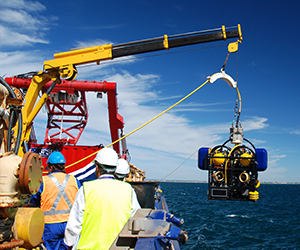
\includegraphics[width=30mm]{Images/ROV_operations_PRODUCT_IMAGE2.jpg}
%		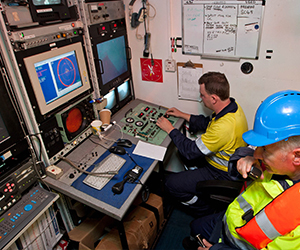
\includegraphics[width=30mm]{Images/ROV_operations_PRODUCT_IMAGE1.jpg}
%		\caption{ROV and its operation, source: www.jfdglobal.com}
%	\label{ROV}
%\end{figure}



\textbf{Methods:}
  \begin{itemize}
  \item
    Postiotion-Based Visual Servo (PBVS) 
  \item
    Image-Based Visual Servo (IBVS)
  \end{itemize}
\textbf{Issues:}
\begin{itemize}
	\item Pose reconstruction
\end{itemize}
\begin{figure}[ht!]
	%\centering
	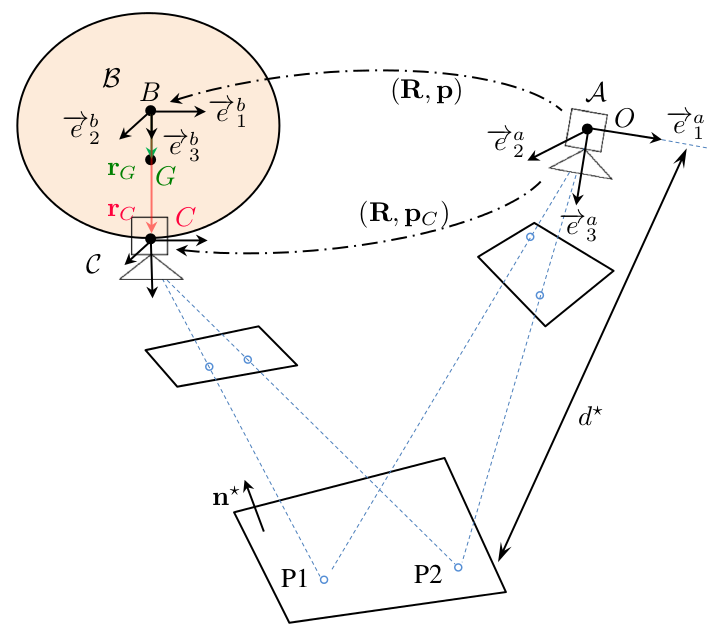
\includegraphics[width=50mm]{Images/Notation.png}
	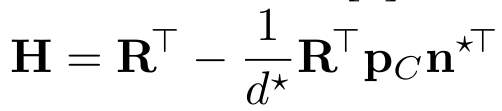
\includegraphics[width=40mm]{Images/Homography.png}
	
	\label{Notation}	
\end{figure}

\end{frame}

\begin{frame}{Kinematic IBVS control}
	\textit{S. Benhimane and E. Malis, 2007:}\\ \textbf{Homography-based 2D visual tracking and servoing}
\begin{itemize}
	\item Kinematic control scheme
	\item No homography decomposition 
\end{itemize}

 
\end{frame}

%\begin{frame}{Stereo camera and full pose reconstruction}
%pose = position + orientation
%
%\textbf{Difficulties:}
%\begin{itemize}
%	\item Short stereo base comparing with long distance to scene 
%\end{itemize}
%
%\end{frame}


%\subsection{Previous Work}

\begin{frame}{Dynamic IBVS control}
\textit{S. Krupinski, G. Allibert, M.-D. Hua and T. Hamel, 2017:}\\ \textbf{An inertial-aided homography based visual servoing control approach for (almost) fully actuated autonomous underwater vehicles}
\begin{itemize}
	\item Dynamic control scheme with cascade inner-outer loop control architecture
\item Linear velocity measured by DVL 
\end{itemize}

\end{frame}

\begin{frame}{Novelty}
Continuation of our previous work. \\
Linear velocity measurement is not required!

Doppler Velocity Log (DVL) is not needed. \\
DVL:
\begin{itemize}
	\item High price
	\item High weight
	\item Violate maximum slope-threshold of DVLs in close proximity operation
\end{itemize}

\end{frame}


\section{Our Contribution}

\subsection{System modeling}

\begin{frame}{Dynamical model}
\end{frame}

\begin{frame}{Model for control design}
Simplifications:
\begin{itemize}
	\item Class of compact-shape AUV
	\item "Munk moment" is neglected
	\item Terms involving Vf are regrouped and considered as disturbance
\end{itemize}
Simplified control model:


\end{frame}



\subsection{Control design}

\begin{frame}{Inner-outer loop control architecture}
Block diagram of the proposed HBVS controller
\begin{figure}
	
\end{figure}

\begin{itemize}
	\item Inner loop:
	\begin{itemize}
		\item Reference angular velocity $$ \Omega_r \stackrel{\triangle}{=}  k_g \mathbf{e}_3 \times \mathbf{R}^{T} \mathbf{e}_3 + \omega_{3r} \mathbf{e}_3$$
		\item Control torque $\Gamma_C$ ensures  $ \Omega \longrightarrow \Omega_r $ 
	\end{itemize} 
	\item Outer loop:
\end{itemize}
\end{frame}

\begin{frame}{Make Titles Informative.}
\end{frame}

\begin{frame}{Make Titles Informative.}
\end{frame}



\section*{Conclusion}

\begin{frame}{Conclusion}

  % Keep the summary *very short*.
  An inertial-aided image-based visual servo controller for the stabilisation of compacted fully actuated AUVs:
  \begin{itemize}
  \item
    %The \alert{first main message} of your talk in one or two lines.
    Using image-based homography without its decomposition.
  \item
    Without relying on linear velocity measurement
  \item
    Locally exponential stability, robustness to unmodeled dynamics and disturbance.
  \end{itemize}
  
  % The following outlook is optional.
  \vskip0pt plus.5fill
  \begin{itemize}
  \item
    A testing campaign is on-going.    
  \end{itemize}
\end{frame}


\begin{frame}
\centering {
	{\huge \textbf{Thank you for your attention!}}	
	{\huge \textbf{Q\&A}}}

\end{frame}



% All of the following is optional and typically not needed. 
%\appendix
%\section<presentation>*{\appendixname}
%\subsection<presentation>*{For Further Reading}
%
%\begin{frame}[allowframebreaks]
%  \frametitle<presentation>{For Further Reading}
%    
%  \begin{thebibliography}{10}
%    
%  \beamertemplatebookbibitems
%  % Start with overview books.
%
%  \bibitem{Author1990}
%    A.~Author.
%    \newblock {\em Handbook of Everything}.
%    \newblock Some Press, 1990.
% 
%    
%  \beamertemplatearticlebibitems
%  % Followed by interesting articles. Keep the list short. 
%
%  \bibitem{Someone2000}
%    S.~Someone.
%    \newblock On this and that.
%    \newblock {\em Journal of This and That}, 2(1):50--100,
%    2000.
%  \end{thebibliography}
%\end{frame}

\end{document}


